\section{簡介}
傳統的語音資訊搜索,基本上都要經過語音辨識系統,轉變成文字,在進行搜尋,然而這種做法的缺點是辨識過程中,不可避免地會出現辨識錯誤、辭典外詞彙而導致辨識結果不準確,進而影響到檢索結果。同時語音文件本身帶有的語音資訊如音高、聲調等等,經過語音辨識系統後,隨即消失了且再也找不回來。所以本章想討論的為利用遞迴類神經網路,分別將語音文件跟查詢對象抽取它們的代表向量,再藉由類神經網路判斷查詢詞是否出現在語音文件中。在本章中,口述詞彙偵測將會被轉化為一個二元分類的問題(Binary
Classification),會希望系統能夠給予一個介於 0~1 的分數(機率值),對於查詢象確實出現在語音文件中的情況給予高分,反之亦然。


\section{利用遞迴式神經網路的查詢詞特徵向量表示法}
\begin{figure}[h]
\centering
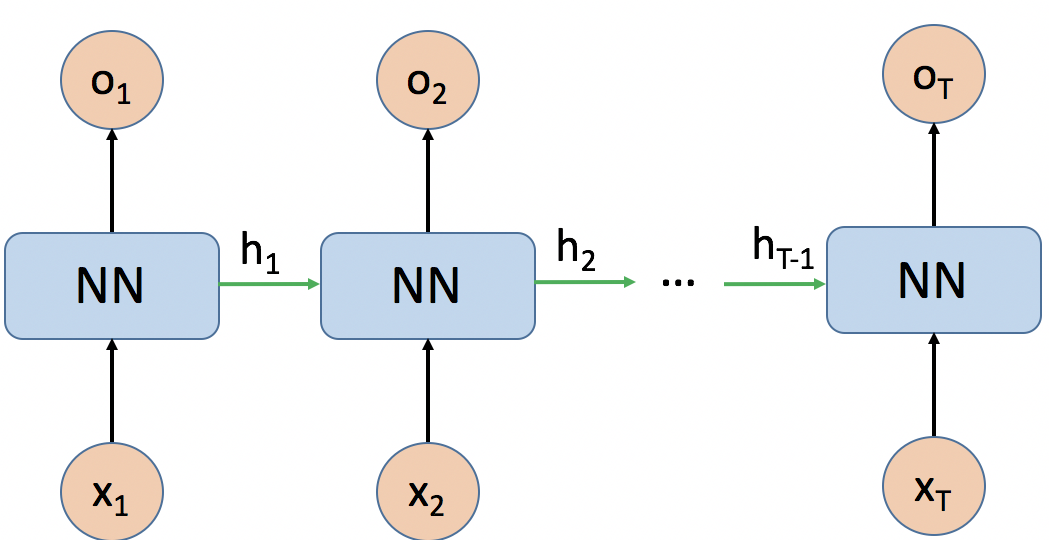
\includegraphics[scale=0.4]{images/ch3_RNN.png} 
\caption{遞迴式類神經網路}
\label{ch3_RNN}
\end{figure}
遞迴式類神經網路因其有記憶性,每個時間點的輸出,會依據之記憶跟現在時間點的輸入改變,如圖~\ref{ch3_RNN}所示。所以依照其特性,可以將語音文件一一給入模型中,在最後的時間點的輸出,可以當做模型已經看過整個語音文件,產生的語音特徵向量。此想法跟序列對序列模型(Sequence-to-Sequence
Model)~\cite{sutskever2014sequence} 的編碼器(encoder)的概念相同,在機器翻譯(Machine
Translation)和自動摘要(Summarization)裡是很常見的模型。在機器翻譯中,會先將欲翻譯的文字先經編碼器(遞迴式類神經網路)編碼成向量。在自動摘要中,也會將整篇文章先經過編碼器變成向量。

